\documentclass[jou]{apa6}

\usepackage[american]{babel}

\usepackage{csquotes}
\usepackage[style=apa,sortcites=true,sorting=nyt,backend=biber]{biblatex}
\DeclareLanguageMapping{american}{american-apa}
\addbibresource{bibliography.bib}


%%%%%%%%%%%%%%%%%%%%%%%%%%%%%%%%%%%%%%%%
%% Discrete Structures
%% The start of RBS stuff
%%%%%%%%%%%%%%%%%%%%%%%%%%%%%%%%%%%%%%%%

% Working internal and external links in PDF
\usepackage{hyperref}
% Extra math symbols in LaTeX
\usepackage{amsmath}
\usepackage{gensymb}
\usepackage{amssymb}
% Enumerations with (a), (b), etc.
\usepackage{enumerate}
\usepackage[framemethod=TikZ]{mdframed}
\usepackage{xcolor}

\let\OLDitemize\itemize
\renewcommand\itemize{\OLDitemize\addtolength{\itemsep}{-6pt}}

\usepackage{etoolbox}
\makeatletter
\preto{\@verbatim}{\topsep=3pt \partopsep=3pt }
\makeatother

% These sizes redefine APA for A4 paper size
\oddsidemargin 0.0in
\evensidemargin 0.0in
\textwidth 6.27in
\headheight 1.0in
\topmargin -24pt
\headheight 12pt
\headsep 12pt
\textheight 9.19in



\title{Sample Quiz 8}
\author{Discrete Structures, Spring 2020}
\affiliation{RBS}

\leftheader{Discrete Sample Quiz 8}

\abstract{%
}

%\keywords{}

\setlength\parindent{0pt}

\begin{document}

%\thispagestyle{empty}

\twocolumn
\section{Quiz 12: Trees}

{\bf Question 1.} The wheel graph $W_4$ has $5$ vertices: 
$4$ vertices form a cycle graph $C_4$ \textendash{} a square; 
one more vertex sits in the middle and is connected with the remaining $4$ vertices. 
($W_4$ is isomorphic to an ordinary Egyptian pyramid.) 
Assume that all vertices in the wheel graph are named with letters and are distinguishable. 
Find the number of unrooted spanning trees in the $W_4$.\\
Write a positive integer in your answer.

\vspace{10pt}
{\bf Question 2.} It is known that a full $m$-ary tree $T$ has $25$ leaves, but the parameter $m$ is 
not known \textendash{} it can take any fixed value: $m = 2,3,4,\ldots$. 
How many inner nodes can $T$ have? Find all possible answers.\\
Write an increasing comma-separated list.

\vspace{10pt}
{\bf Question 3.}\\ There is a rooted tree with $111$ vertices and each vertex can have up to $3$ children. 
Find the minimum and the maximum height of this tree.\\
Write two comma-separated integers.


\vspace{10pt}
{\bf Question 4.}\\ 
Assume that there is a rooted tree (with anonymous/unnamed vertices and unordered children) and its vertices have 
the following degrees $3, 3, 2, 2, 1, 1, 1, 1$. It is also known that its root vertex has $3$ children. 
Find the number of such rooted unordered trees.\\
Write a positive integer.


\vspace{10pt}
{\bf Question 5.}

\begin{figure}[!htb]
\center{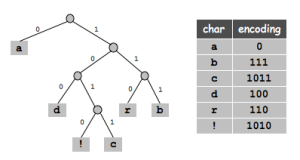
\includegraphics[width=3.2in]{quiz-12/huffman-tree.png}}
\caption{\label{fig:huffman-tree} Encoding with a Tree.}
\end{figure}

Figure~\ref{fig:huffman-tree} shows an efficient method to send messages
(like {\tt abracadabra!}) using $6$ characters.
Assume that the characters appear with the following probabilities:\\
{\small
\begin{tabular}{|l|c|c|c|c|c|c|} \hline
Symbol & {\tt a} & {\tt b} & {\tt d} & {\tt r} & {\tt c} & {\tt !} \\ \hline
Probability &  $1/2$ & $1/8$ & $1/8$ & $1/8$ & $1/16$ & $1/16$ \\ \hline
\end{tabular}\\
}
Find the expected number of bits used per character (i.e. $E(X)$ \textendash{} the expected value of
the random variable $X$, which describes the number of bits used per one
character from this random distribution.)\\
Write a real number \textendash{} the number of bits rounded to the nearest thousandth.

%{\em Note.} For the given probabilities, this tree offers the best compression
%(using it for the encoding needs the smallest 
%expected number of bits). For such optimal codes we say that the expected number of bits
%for sending one character equals the {\em entropy} of the probability distribution.
%It is fine, if the entropy is a fractional (non-integer) number of bits.



 
 


\vspace{10pt}
{\bf Question 6.} 
The string
$$\rightarrow\;\rightarrow\;\rightarrow\;\rightarrow\;\rightarrow\;a\;b\;\textcolor{red}{\triangle}\;\neg\;c\;\neg\;d\;c\;e\;\rightarrow\;\neg\;a\;\rightarrow\;d\;e.$$
is the prefix notation for a Boolean logic expression with one symbol replaced by a $\textcolor{red}{\triangle}$. 
What can this $\textcolor{red}{\triangle}$ represent?\\
{\bf (A)} It is a propositional variable ($a,b,c$ or similar).\\
{\bf (B)} It is a unary Boolean operator ($\neg$ or similar).\\
{\bf (C)} It is a binary Boolean operator ($\rightarrow$ or similar).\\
{\bf (D)} It cannot be any of these; the expression is invalid in all these cases.

Write the answer letter (A, B, C, or D).



\vspace{10pt}
{\bf Question 7.} 
Imagine that you search for all ways how to place $4$ queens on a $4 \times 4$ chessboard so that 
they do not attack each other. (A chess queen attacks all squares on its horizontal, on its vertical
and also on both diagonals.)\\
Imagine that you build a tree for this:\\
{\bf (Level 0 to Level 1)} The root of the tree is an empty $4 \times 4$ chess-board; you add to it four children 
(all $4$ ways how you can place a queen on the 1st row of the chess-board).\\
{\bf (Level 1 to Level 2)} For any of the vertices you added in the previous step, add children on level $2$ by placing 
another queen on the 2nd row so that it does not attack the first one.\\
In general, the vertex on level $L=i$ has queens on rows $1,\ldots,i$ that do not attack each other. 
Any vertex on level $L=4$ will be a solution to this ``4 queens problem'' with all four rows containing a queen.

Write the total number of vertices in this tree (that the backtracking algorithm will visit).


\vspace{10pt}
{\bf Question 8.} An undirected graph $G = (V,E)$ has the set of vertices $V$ \textendash{} 
the set of all positive divisors of the number $900$ (including $1$ and $900$ itself).
A pair of divisors $(d_1,d_2)$ is an edge in $G$ iff their ratio
$d_1/d_2$ (or $d_2/d_1$) is a prime number.

In the root vertex $v_1=1$ we start the BFS (Breadth-first-search) traversal of the graph $G$. For every vertex 
we visit all its adjacent vertices in increasing order (for example edges $(1,2)$, $(1,3)$ and $(1,5)$ 
are visited in this order. When all the children of vertex $1$ are visited, 
we start visiting all the adjacent vertices of $v_2=2$, and so on.). We get the BFS traversal order like this:
$$v_1=1,\,v_2=2,\,v_3=3,\,v_4=5,\,v_5=4,\,\ldots$$
Find the vertices $v_{13},\,v_{14},\,v_{15}$ in this BFS order.

Write three comma-separated numbers.

%\newpage
\vspace{10pt}
{\bf Question 9.}

\begin{figure}[!htb]
\center{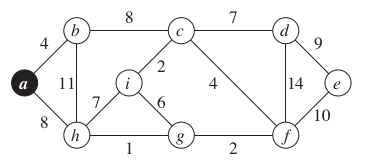
\includegraphics[width=2in]{quiz-12/prim-algorithm.png}}
\caption{\label{fig:prim-algorithm} Weighted Graph.}
\end{figure}


Find the weight of a minumum spanning tree (MST) in the tree shown in Figure~\ref{fig:prim-algorithm}. 
In order to construct this tree, you can use Prim's algorithm (Rosen2019, p.836). 
Start in vertex $a$ - this is your first tree $T_1$. 
In every step pick the minimum weight edge that is adjacent to $T_i$ (and does 
not create any loop) \textendash{} add it to the tree $T_i$, and obtain the next 
tree $T_{i+1}$. Continue adding the minimum weight edges until all vertices are connected.
(In the second step you will have a choice 
to add $(b,c)$ or $(a,h)$ as both edges have the same weight $8$. There may be several MSTs
in a graph, but all of them will have the same total weight.)

Write the total MST weight as a number.


\vspace{10pt}
{\bf Question 10.}
The vertices in the directed graph (Figure~\ref{fig:dfs-traversal2}) are visited in the DFS
order. You start with the alphabetically smallest vertex ($q$), order all the vertices connected to it
alphabetically, then build the DFS traversal. 

\begin{figure}[!htb]
\center{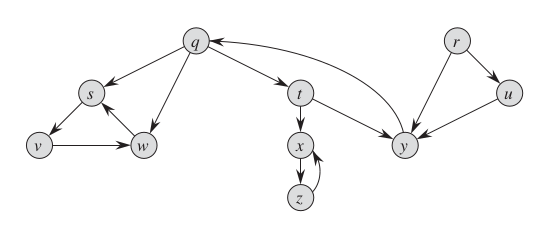
\includegraphics[width=3in]{quiz-12/dfs-traversal2.png}}
\caption{\label{fig:dfs-traversal2} Graph for DFS traversal.}
\end{figure}




Write the sequence with parentheses and vertices for the graph 
on Figure 3 \textendash{} similar to the sequence (\ref{eq:dfs-search-order}) \textendash{} see Appendix. 
Each of its $10$ vertices should be mentioned in your 
traversal order twice (the first time with an opening parenthesis, the second time 
with a closing parenthesis).




\mbox{}
\newpage

{\bf Appendix: DFS}

\begin{figure}[!htb]
\center{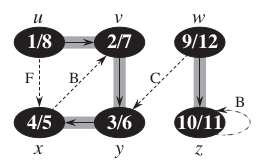
\includegraphics[width=1.4in]{quiz-12/dfs-traversal.png}}
\caption{\label{fig:dfs-traversal} Sample DFS traversal.}
\end{figure}

Figure~\ref{fig:dfs-traversal} shows a DFS (Depth-First-Search) traversal
in a directed graph. Vertexes are visited in alphabetical order 
(so $u$ is visited first; followed by its alphabetically first 
child $v$, followed by $y$, followed by $x$. After that
we visit another tree (unreachable from the first one) \textendash{}
$w$ followed by $z$.)\\
{\bf Tree edges} that belong to the DFS traversal tree are shaded;\\
{\bf Back edges} that point back from a vertex to its ancestor in the tree (or a loop to itself)
are labeled by $B$;\\
{\bf Forward edges} that jump from a vertex to its descendant in the DFS tree (other than a child) are
labeled by $F$;\\
{\bf Cross edges} that jump between two vertices that are not descendants/ancestors of 
each other are labeled by $C$.

The following sequence
\begin{equation} \label{eq:dfs-search-order}
\textcolor{blue}{\mathtt{(u\;(v\;(y\;(x\;x)\;y)\;v)\;u)\;(w\;(z\;z)\;w)}}
\end{equation}
denotes the DFS traversal order in the oriented graph. 
Every time when we enter some vertex (and its subtree), 
we open a parenthesis and write the vertex name; when we leave, 
we write the vertex name again and close the parenthesis.\\
This order is also written inside each vertex (for example {\tt 1/8} 
for vertex $u$ means that we entered it in Step 1, and left it in 
Step 8). For vertex $z$ this pair is {\tt 10/11} (we entered this leaf
of the DFS tree and immediately left it).
%\end{mdframed}


%\begin{mdframed}[roundcorner=6pt]
%\section{Appendix 2: Prim's Algorithm}

%\end{mdframed}

\newpage
\subsection{Answers}

\vspace{4pt}
{\bf Question 1.} Answer: {\tt 45} \\

There are only three kinds of trees with $5$ vertices, if isomorphic trees count as the same. 
See {\em isomers of pentane} \textendash{} \url{https://bit.ly/2W4BWiw} (either the vertex degrees are 
$1,2,2,2,1$, or $1,2,3,1,1$, or $4,1,1,1,1$).

Let us denote the vertices by $A,B,C,D,E$ ($E$ being the vertex at the top of the pyramid). 
The only non-existing edges are $(A,C)$ and $(B,D)$ (otherwise it is almost like $K_5$). 
In Figures~\ref{fig:spanning-trees-on-w5-a}, \ref{fig:spanning-trees-on-w5-b}, 
\ref{fig:spanning-trees-on-w5-c} we show different subcases depending 

\begin{figure}[!htb]
\center{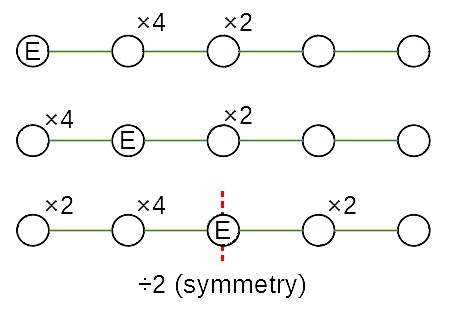
\includegraphics[width=2.2in]{quiz-12/spanning-trees-on-w5-a.png}}
\caption{\label{fig:spanning-trees-on-w5-a} 24 trees with all degrees $\leq 2$.}
\end{figure}

\begin{figure}[!htb]
\center{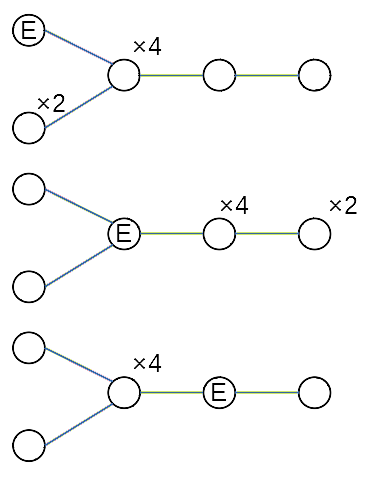
\includegraphics[width=1.8in]{quiz-12/spanning-trees-on-w5-b.png}}
\caption{\label{fig:spanning-trees-on-w5-b} 20 trees with one degree $=3$.}
\end{figure}

\begin{figure}[!htb]
\center{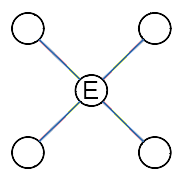
\includegraphics[width=0.9in]{quiz-12/spanning-trees-on-w5-c.png}}
\caption{\label{fig:spanning-trees-on-w5-c} 1 tree with one degree $=4$.}
\end{figure}

$$N = (8 + 8 + 8) + (8 + 8 + 4) + (1) = 45.$$


\vspace{4pt}
{\bf Question 2.} Answer: {\tt 1,2,3,4,6,8,12,24} \\
In a full $m$-ary tree initially there is just one 
node (it is the root and also a leaf). After that
the number of leaves can increase by $m-1$ in a single step 
(one leaf becomes an internal node and creates exactly $m$ children). 
The question now becomes \textendash{} in how many arithmetic
progressions both numbers $1$ and $25$ participate. 
We get these variants:

$$\left\{ \begin{array}{l}
1,2,3,\ldots,25 \\
1,3,5,7,9,11,13,15,17,19,21,23,25 \\
1,4,7,10,13,16,19,22,25 \\
1,5,9,13,17,21,25 \\
1,7,13,19,25 \\
1,9,17,25 \\
1,13,25 \\
1,25 \\
\end{array} \right.$$

In each variant we count the number of increments
(how many times $m-1$ was added in order to get $25$). At every such step 
an inner node is created.
The number of inner nodes can be computed as $\frac{25-1}{m-1}$. 

\begin{tabular}{|l|l|} \hline
$m$ & Inner nodes \\ \hline
$2$ & $24$ \\ \hline
$3$ & $12$ \\ \hline
$4$ & $8$ \\ \hline
$5$ & $6$ \\ \hline
$7$ & $4$ \\ \hline
$9$ & $3$ \\ \hline
$13$ & $2$ \\ \hline
$25$ & $1$ \\ \hline
\end{tabular}





\vspace{4pt}
{\bf Question 3.} Answer: {\tt 4,110}

{\bf Minimum height.} There is one vertex (the root) at depth $d=0$, 
at most $3$ vertices at $d=1$, at most $9$ vertices at $d=2$, 
at most $27$ vertices at $d=3$ and at most $81$ vertices at $d=4$. 
If maximum depth is $4$ (i.e. the height of the tree is also $4$), then 
there can be at most $1 + 3 + 9 + 27 + 81 = 121$
vertices in the tree. Which is just fine, since $111 < 121$. 

{\bf Maximum height.} In this case each vertex has just one child. 
The deepest node has depth $d=110$ (one less than the number of nodes
in the tree). 


\vspace{4pt}
{\bf Question 4.} Answer: {\tt 6}

We can sort cases depending on the location of the other vertex $v_1$
with degree $3$ (it is known that another one is root; let us denote the root by $v_0$).
That other vertex can have depth $1$, $2$ or $3$.  

{\bf Case 1.} $\text{depth}(v_1) = 1$. There are three possible trees in this case; 
the two vertices of degree $2$ can be either both children of $v_0$, or both of $v_1$, 
or one can be a child of $v_1$, and another of $v_0$.\\
{\bf Case 2.}  $\text{depth}(v_1) = 2$. There are two possible trees in this case; 
one of the vertices of degree $2$ is beteween $v_0$ and $v_1$; but another vertex
of degree $2$ can be a child of $v_0$, or a child of $v_1$.\\
{\bf Case 3.} $\text{depth}(v_1) = 3$. There is just one tree in this case. 
Both vertices of degree $2$ are between $v_0$ and $v_1$. 






\vspace{4pt}
{\bf Question 5.} Answer: {\tt 2.125} \\
To geet the expected value of the random variable (the length of the code in bits)
multiply the respective code lengths for all six letters of the alphabet
by their respective probabilities: 

$$1 \cdot \frac{1}{2} + 3 \cdot \frac{1}{8} + 3 \cdot \frac{1}{8} + 3 \cdot \frac{1}{8} + 4 \cdot \frac{1}{16} + 4 \cdot \frac{1}{16} = 2\frac{1}{8}.$$

{\em Note.} Variable length codes where one code is never a prefix of another and
all the codes can be arranged in a binary tree, where grouping them starts by the two least frequent letters
({\tt !} and {\tt c} in our case) is named {\em Huffman tree}. 

\vspace{4pt}
{\bf Question 6.} Answer: {\tt C}\\
In any (infix, prefix or postfix) expression the number of binary operators (in our case the only 
such operator is $\rightarrow$) should be one less than the number of operands (in our case 
these are the Boolean variables $a$,$b$,$c$,$d$,$e$). Unary operators (in our case $\neg$) do not count. 

In our expression so far there are $7$ operators $\rightarrow$. There are also $9$ Boolean variables. 
Therefore the triangle should become a binary operator $\rightarrow$. 
The expression looks like this: 
$$\rightarrow\;\rightarrow\;\rightarrow\;\rightarrow\;\rightarrow\;a\;b\;\textcolor{red}{\rightarrow}\;\neg\;c\;\neg\;d\;c\;e\;\rightarrow\;\neg\;a\;\rightarrow\;d\;e.$$

Here is the regular (infix) representation of the same Boolean expression:

{\footnotesize
$$((((a \rightarrow b) \rightarrow (\neg c \textcolor{red}{\rightarrow} \neg d)) \rightarrow c) \rightarrow e) 
  \rightarrow (\neg a \rightarrow (d \rightarrow e)).$$
}

\vspace{4pt}
{\bf Question 7.} Answer: {\tt 17}\\

If we denote the rows/horizontals by numbers $1,2,3,4$ and the columns/verticals by letters $A,B,C,D$
as in ordinary chess, we can denote adding queens in the tree shown in Figure~\ref{fig:backtracking-4-queens}. 
The only two solutions are two shaded nodes at the bottom. All other placements of queens are 
dead ends. 

{\em Note.} Not pursuing these dead ends (not going deeper, if we know that it is useless) 
reduces the number of nodes to consider to $17$ (down from $4! = 24$ or even $4^4 = 256$, if we would
apply {\em brute force}). This is not very much, but for larger chess boards the savings are larger.
See \url{https://bit.ly/3aQ1feo}.

\begin{figure}[!htb]
\center{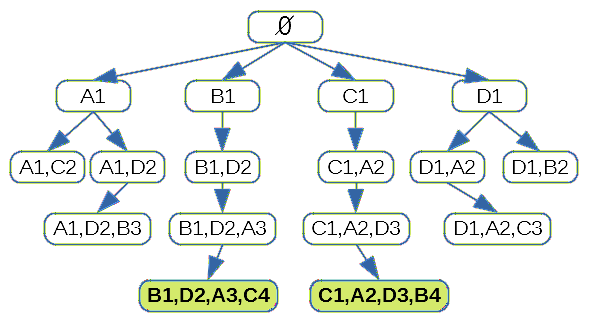
\includegraphics[width=2.4in]{quiz-12/backtracking-4-queens.png}}
\caption{\label{fig:backtracking-4-queens} Backtracking tree: 4 Queens problem.}
\end{figure}


\vspace{4pt}
{\bf Question 8.} Answer: {\tt 18,30,50} \\

You can determine the order of the vertices in the BFS traversal by counting vertices
layer by layer (Figure~\ref{fig:divisors-of-900}). 
Note that the number $30 = \sqrt{900}$ is the $14$th vertex in the BFS traversal (it is in the very middle). 

\begin{figure}[!htb]
\center{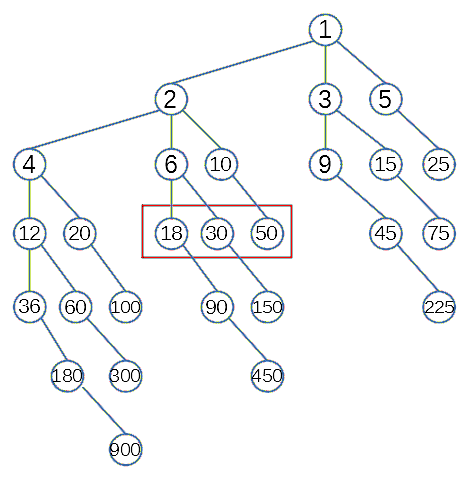
\includegraphics[width=2in]{quiz-12/divisors-of-900.png}}
\caption{\label{fig:divisors-of-900} BFS tree with divisors of 900.}
\end{figure}



\vspace{4pt}
{\bf Question 9.} Answer: {\tt 37} \\

We add edges using Prim's algorithm: 

\begin{tabular}{|l|l|l|} \hline
Step 1 & $AB$ & 4 \\ \hline
Step 2 & $BC$ & 8 \\ \hline
Step 3 & $CI$ & 2 \\ \hline
Step 4 & $CF$ & 4 \\ \hline
Step 5 & $FG$ & 2 \\ \hline
Step 6 & $GH$ & 1 \\ \hline
Step 7 & $CD$ & 7 \\ \hline
Step 8 & $DE$ & 9 \\ \hline
\end{tabular}


Total weight: 

$$4 + 8 + 2 + 4 + 2 + 1 + 7 + 9 = 37.$$


\vspace{4pt}
{\bf Question 10.} Answer:\\

$$\textcolor{blue}{\mathtt{(q\,(s\,(v\,(w\;w)\,v)\,s)\,(t\,(x\,(z\;z)\,x)\,(y\,y)\,t)\,q)\;\;(r\,(u\;u)\,r)}}$$

The DFS traversal creates two trees 
with $q$ and $r$ as their roots respectively.

\end{document}

